%!TEX root = ../main.tex

\subsection{Vacromium}
\label{ssec:vacromium}

Next, a vacromium absorber is placed in the beam path\footnote{The vacromium
Mössbauer spectrum was measured last during the lab exercise. To streamline the text
it is however decided to discuss the material already here.}. The analysis of data
proceeds as is presented in \autoref{ssec:iron}. One absorption peak can be
discovered in the vacromium Mössbauer spectrum as seen in \autoref{fig:vacromium} and
\autoref{tab:vacromium}.



\begin{figure}
	\centering
	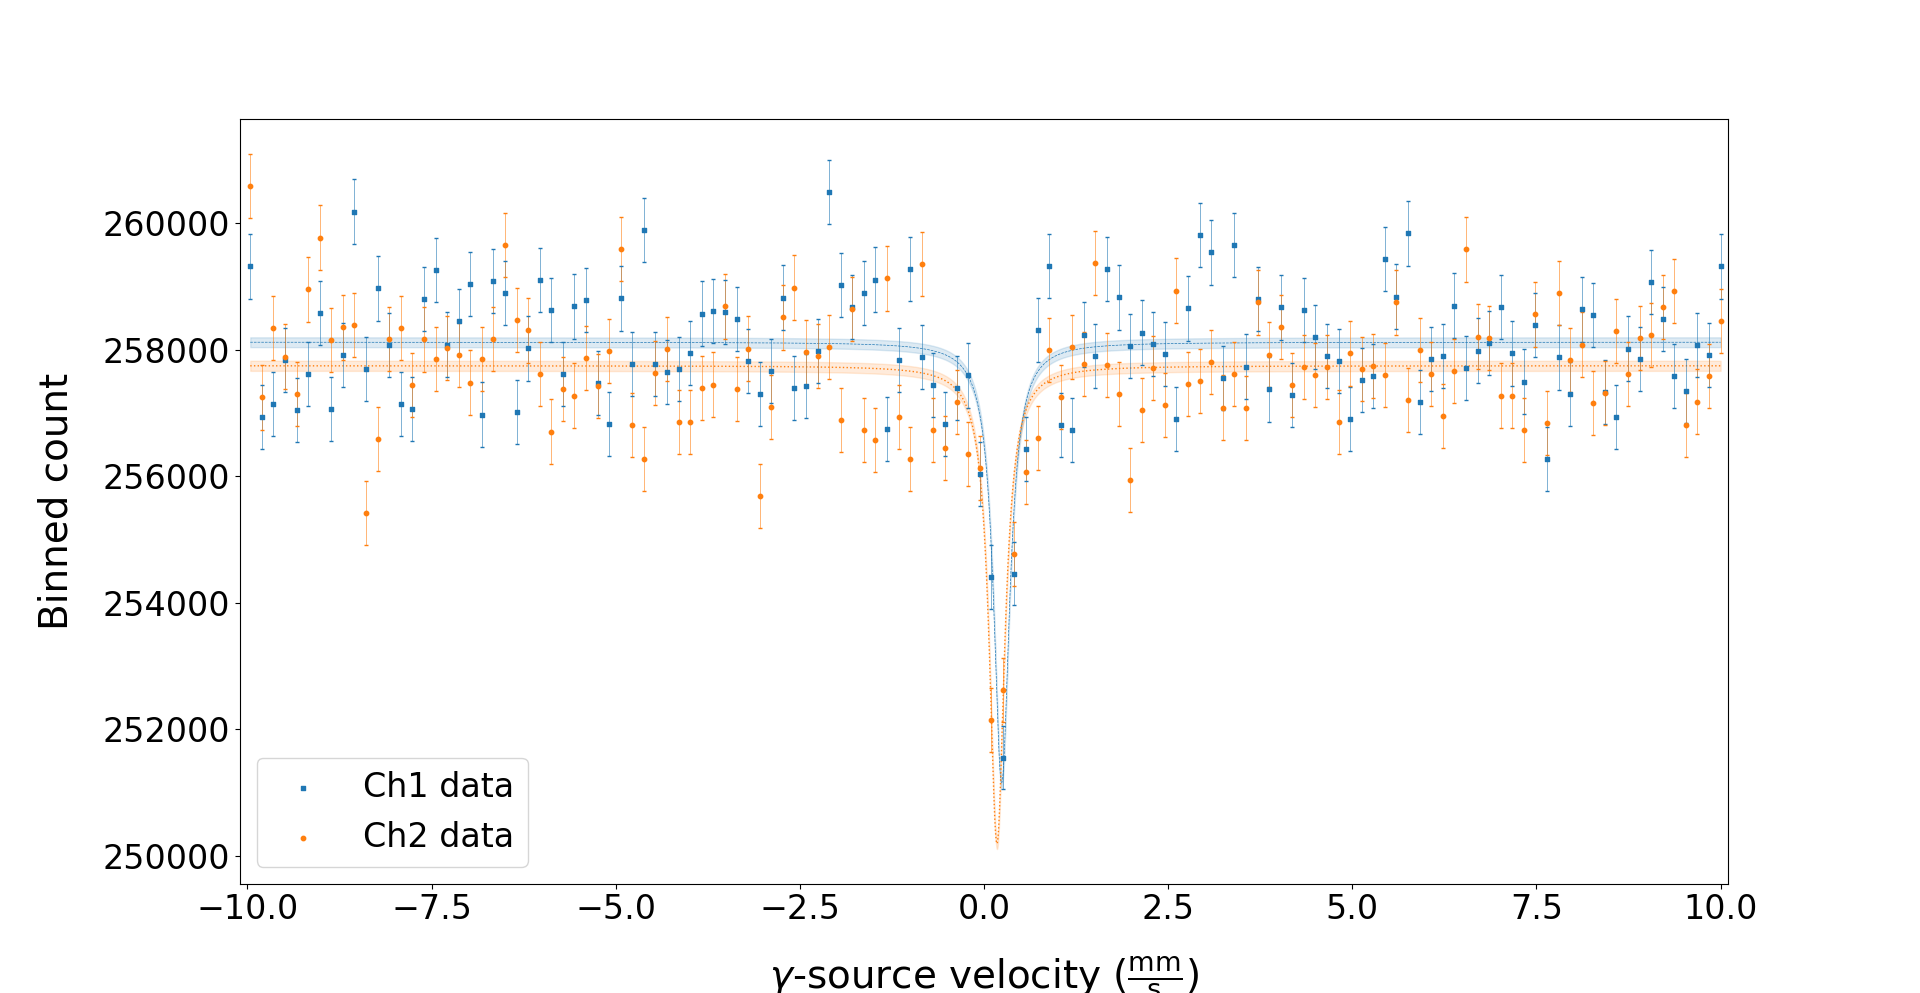
\includegraphics[width=1.0\textwidth]{./fig/Vacromium.png}
	\caption{Mössbauer spectrum of vacromium}
	\label{fig:vacromium}
\end{figure}

\begingroup
\renewcommand{\arraystretch}{1.3}
\begin{table}
	\begin{center}
	\caption{Mössbauer spectrum fit parameters for vacromium}
	\begin{tabular*}{0.9\textwidth}{@{\extracolsep{\fill}} c|ccccc}
  \toprule
	\hline
  Peak \# & $\Upphi_0$ & $A$ & $v_0$ & $\Gamma$ & Channel \\
	\hline
  \multirow{2}{*}{\#1} & $258122\pm78$ & $120\pm39.1$ & $0.24\pm0.03$ & $0.262\pm0.050$ & Ch1 \\
                       & $257749\pm80$ & $120\pm54.1$ & $0.18\pm0.01$ & $0.252\pm0.082$ & Ch2 \\
                       \hline
    \bottomrule
		\end{tabular*}
		\label{tab:vacromium}
	\end{center}

\end{table}
\endgroup

